Dans la litt\'erature, le {\em line-graphe} est d\'esign\'e par le {\em graphe adjoint} ou {\em linegraph}. 

\begin{definition}
Soit $G=(V,A)$ un DAG. 
Le line-graphe de $G$ est un graphe non-orient\'e $L(G) = (V',E)$ o\`u $V'=A$ et une paire $[a,a']$ de sommets de $L(G)$ est une ar\^ete ssi $a$ et $a'$ ont une extremit\'e commun (peu importe l'extremit\'e initial ou finale comme dans la figure \ref{typeSommetsEnCommun}) dans $G$.
\end{definition}

\begin{figure}[htb!]\vspace{-0.5em}
	\centering
	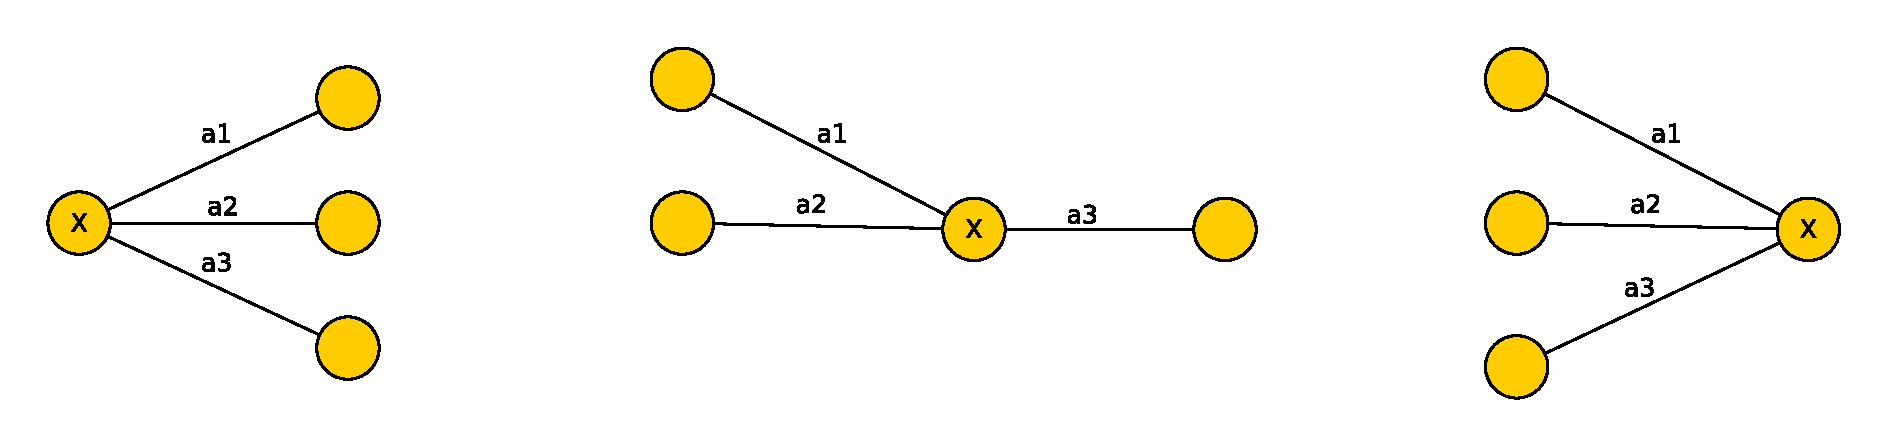
\includegraphics[scale=0.50]{typeSommetsEnCommun.eps}\vspace{-0.5em}
	\caption{ Sommet $X$ partag\'e entre les ar\^etes. De la gauche vers la droite : sommet entrant, \`a droite sommet interm\'ediaire et sommet sortant }\vspace{-0.5em}
	\label{typeSommetsEnCommun}
\end{figure}

Avec $G$ ayant $n$ sommets et $m$ arcs, le graphe $L(G)$ a $m$ sommets et $E$ ar\^etes dont 
$$ E = \sum_{i=1 }^{n} d_i(d_i -1)/2$$, 
$d_i$ \'etant le degr\'e de chaque sommet $i$ de $G$.
Le graphe $G$ est  appel\'e le {\em graphe racine} de $L(G)$. 
Un exemple de graphe racine et son line graphe est present\'e dans la figure \ref{rootGrapheLineGrapheExemple}

\begin{figure}[htb!]\vspace{-0.5em}
	\centering
	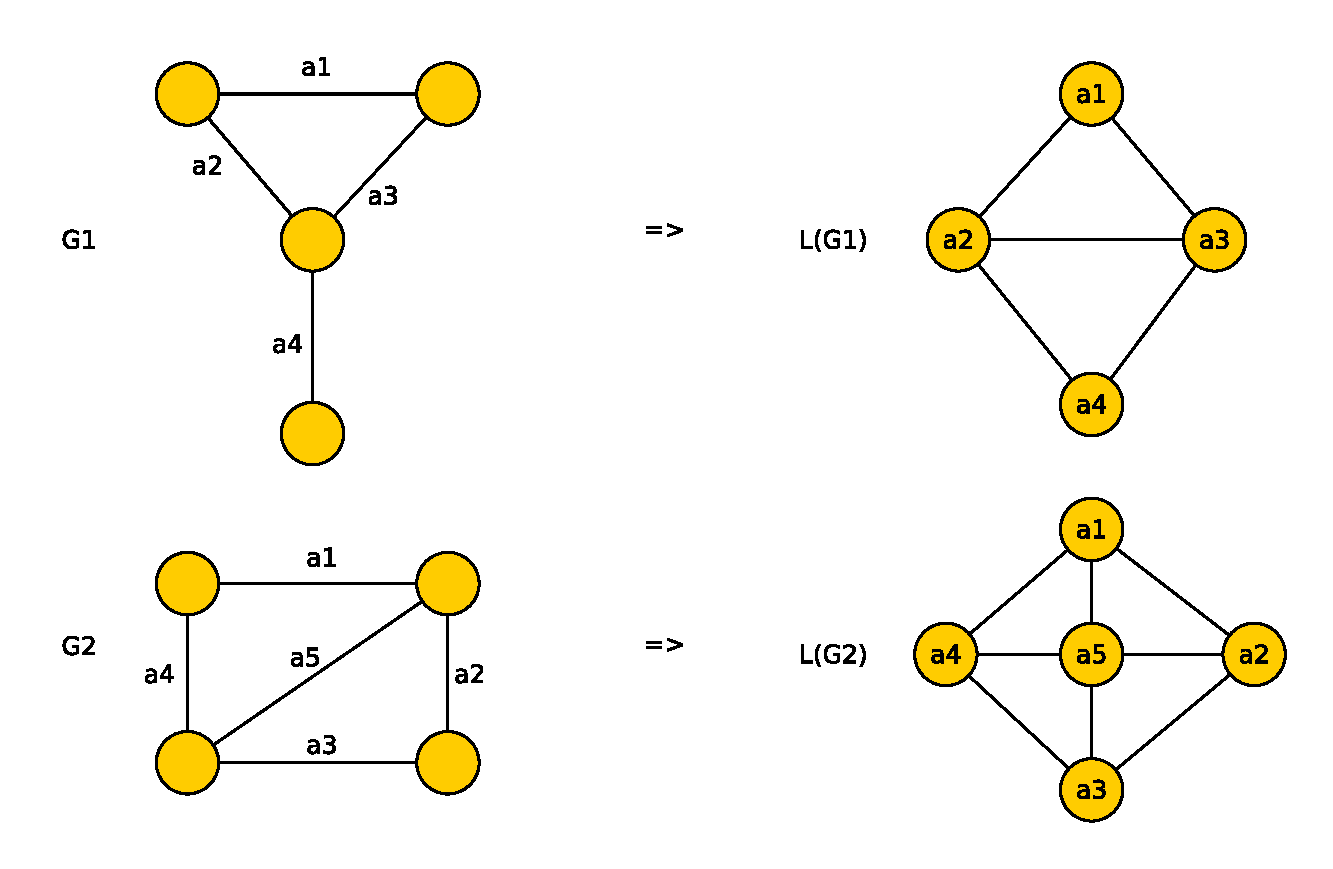
\includegraphics[scale=0.50]{rootGrapheLineGrapheExemple.eps}\vspace{-0.5em}
	\caption{ Le graphe racine $G$ et son line graphe L(G) }\vspace{-0.5em}
	\label{rootGrapheLineGrapheExemple}
\end{figure}

La notion de line-graphe a \'et\'e introduite par {\em Whitney} \cite{isomorphismeLineGraphe} \`a partir de l'isomorphisme d'ar\^etes. Il montra que l'isomorphisme des ar\^etes implique l'isomorphisme de graphes connexes \`a condition que ces graphes connexes soient diff\'erent de $K_{1,3}$(graphe \'etoile) et $K_3$(graphe triangle).
\begin{proposition}
Le graphe \'etoile $K_{1,3}$ n'est pas un {\em line graphe}.
\end{proposition}
\begin{proof}
Supposons que $K_{1,3}$ est le line graphe de $H$ ($K_{1,3} = L(H)$). 
Alors $H$ est un graphe connexe de quatre ar\^etes.
Tous les graphes connexes de quatres ar\^etes sont repr\'esent\'es dans la figure  \ref{graphesRacinesDeQuatresAretes}. 
Comme $L(C_4) = C_4$  et $L(K_{1,3} + e) = K_4 + e$ (voir figure \ref{rootGrapheLineGrapheExemple}), $L(H)$ ne peut \^etre que l'un des trois arbres $P_4$, $K_{3,2}$ et $K_{1,4}$.
Ce qui est contraire \`a notre hypoth\`ese de d\'epart ($K_{1,3} = L(H)$).
\end{proof}

\begin{figure}[htb!]\vspace{-0.5em}
	\centering
	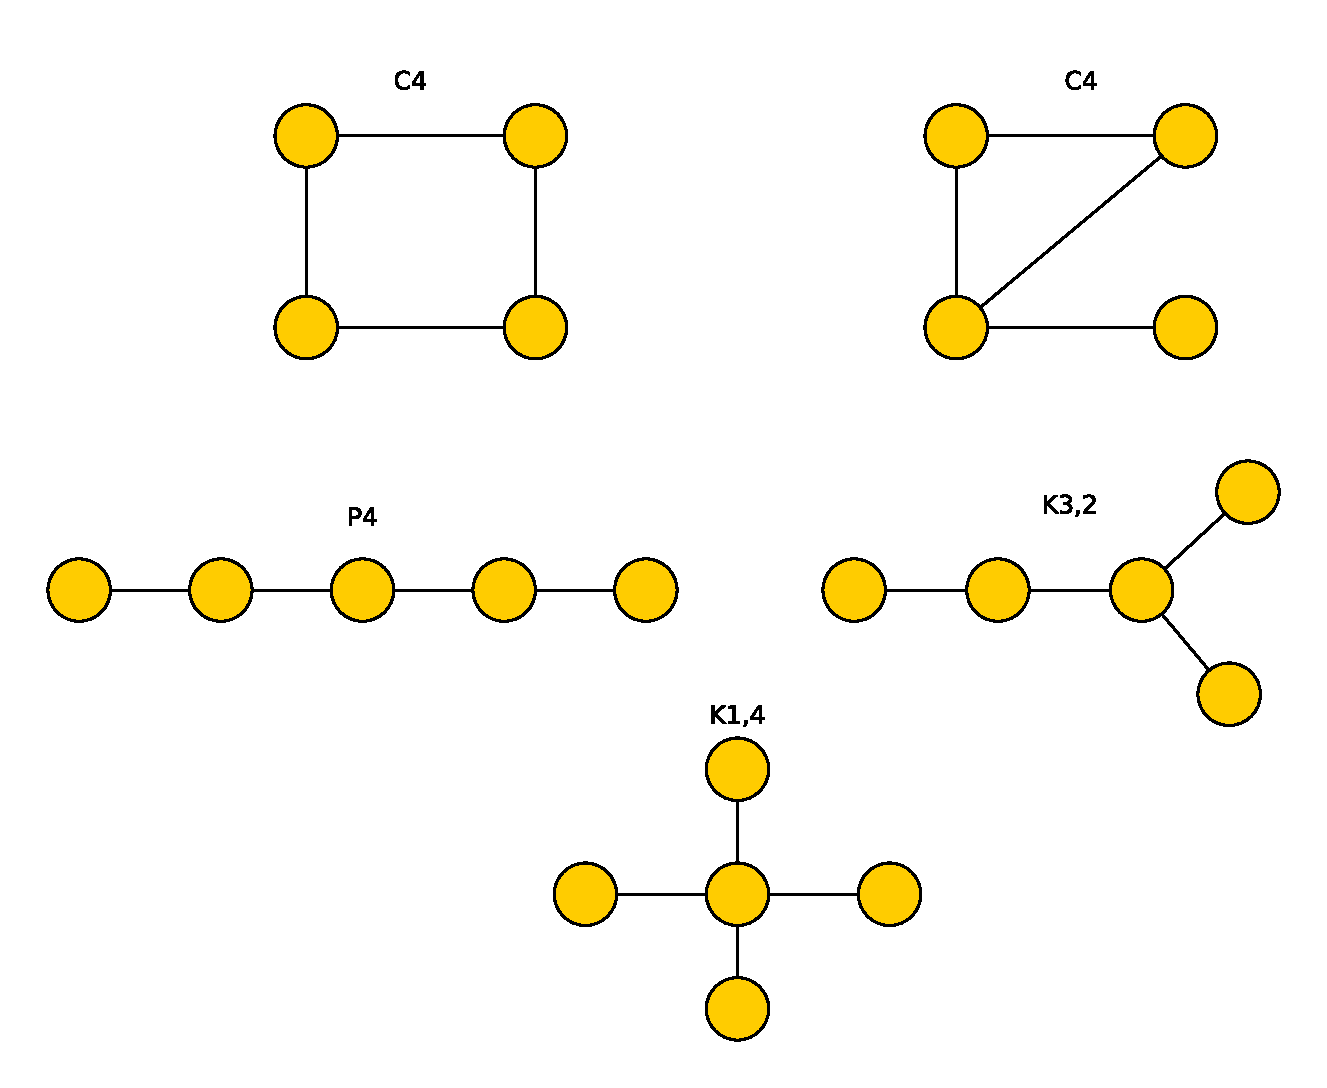
\includegraphics[scale=0.50]{graphesRacinesDeQuatresAretes.eps}\vspace{-0.5em}
	\caption{ Les graphes racines possibles de $K_{1,3}$ de quatres ar\^etes   }\vspace{-0.5em}
	\label{graphesRacinesDeQuatresAretes}
\end{figure}

Le graphe \'etoile ($K_{1,3}$) joue un r\^ole important dans la caracterisation des line-graphes.
La premi\`ere propri\'et\'e, provient de {\em Krausz} \cite{krausz1943demonstration} et est relatif au partitionnement du line-graphe en sous-graphes. La seconde, edit\'e par {\em van Rooij and wilf} \cite{ROOIJetWILF1965interchange}, d\'ecrit la structure de base d'un graphe pour \^etre un line-graphe. Et enfin {\em Beineke\cite{beineke1968derived} et Hemminger}   affichent les neufs sous-graphes ne pouvant pas avoir de line graphes. decoule
\begin{theorem}
\label{caracteristiquesLinegraphes}
Soit $H$ un line-graphe. Les affirmations suivantes sont \'equivalentes.
\begin{itemize}
	\item les ar\^etes de $H$ peuvent \^etre partition\'ees en sous graphes complets tel que aucun sommet est contenu dans plus de deux sous-graphes. Ces sous graphes complets sont des cliques.
	\item $H$ ne contient pas $K_{1,3}$ comme sous-graphe et si deux triangles ont une ar\^ete commune alors le sous graphe induit est $K_4$.
	\item Aucun des neufs sous-graphes de la figure \ref{neufSousGraphesInterditDesLineGraphes} ne peut \^etre un sous graphe d'un line graphe $G$.
\end{itemize}
\end{theorem}

\begin{figure}[htb!]\vspace{-0.5em}
	\centering
	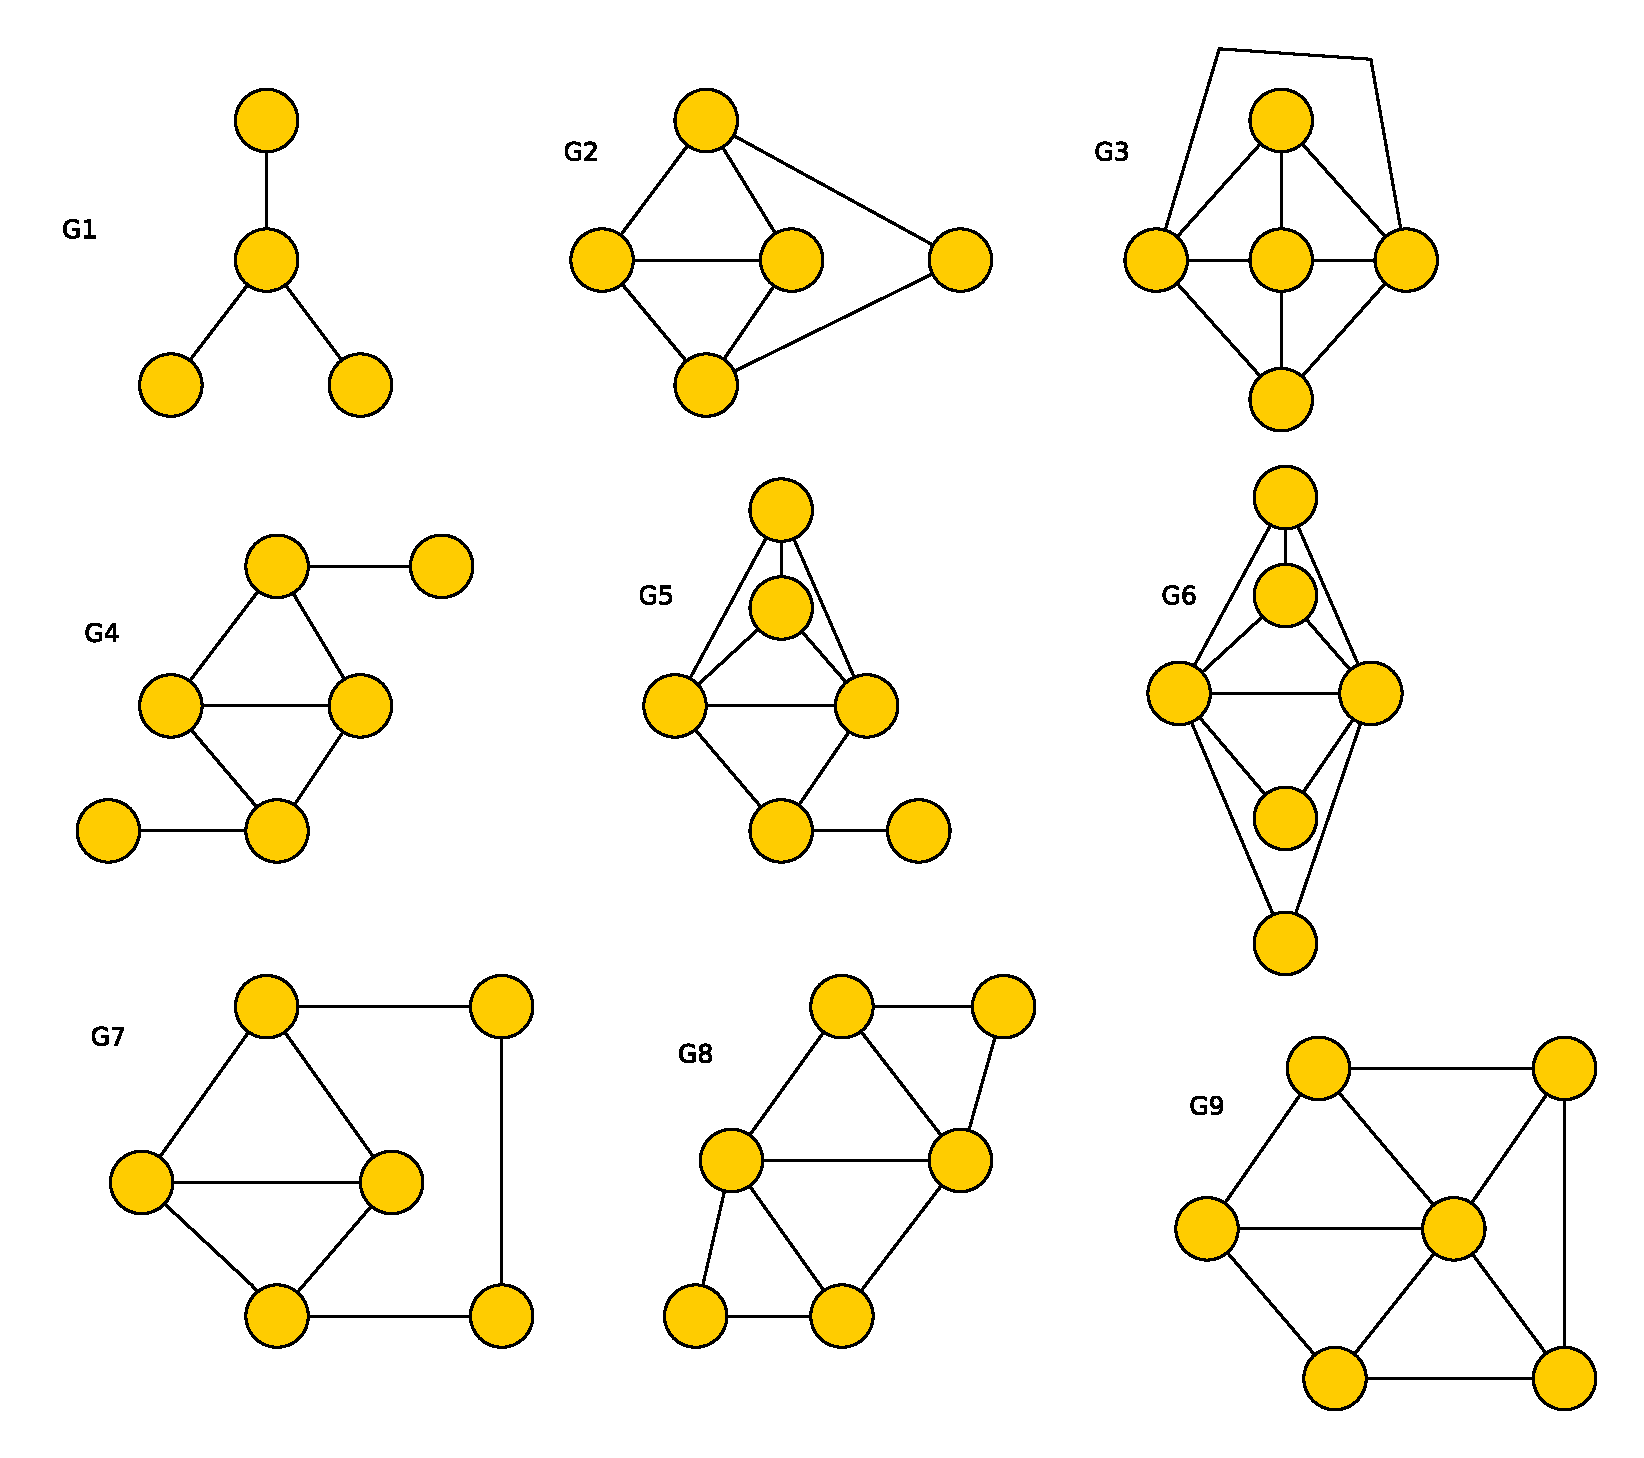
\includegraphics[scale=0.50]{neufSousGraphesInterditDesLineGraphes.eps}\vspace{-0.5em}
	\caption{ Line graphes et sous graphes interdits }\vspace{-0.5em}
	\label{neufSousGraphesInterditDesLineGraphes}
\end{figure}

\begin{proof}
Voir theor\`eme 8.4, chapitre 8 \cite{lineGraphe}.
\end{proof}
